\section{Hardware}

\subsection{Grundlagen}
\label{sec:basics}

\subsubsection{Arten von VR Headsets}
\label{sec:vr-headset-types}

Bei VR Headsets werden grundsätzlich drei verschiedene Arten unterschieden:

\begin{itemize}
    \item Tethered Headsets
    \item Standalone Headsets
    \item Smartphone und Handheld Headsets
\end{itemize}

In Folge werden diese Arten kurz beschrieben, sodass die beschreibungen von der Technologien verstanden werden können.
Für eine genauere beschreibung dieses Themas wird auf~\cite{ANIWAA_TEAM_2021} verwiesen.

\emph{Tethered VR Headsets} müssen immer mit einem Computer verbunden sein, weil die VR-Applikation ausschließlich auf dem Computer läuft.
Die Brille hat dabei einerseits die Funktion die vom Computer gerenderten daten darzustellen und andererseits Positionsdaten an den Computer zurückzusenden, damit diese in der Applikationslogik verwendet werden können, um zukünftige Bilddaten zu rendern.

Bei \emph{Standalone VR Headsets} ist in der Brille ein Computer integriert, auf welchem die VR Applikation läuft.
Der Computer dient ausschließlich aus Entwicklungsplattform und die fertigen Applikationen müssen auf die Brille heruntergeladen werden.

Im Falle des \emph{Smartphone VR Headsets} läuft die Applikation auf einem Smartphone.
Um die Immersion zu erhöhen wird das Smartphone in die VR-Brille eingeschoben.
In diesem Fall dient das Telefon sowohl als Anzeigegerät als auch als Sensordatenprovider.
Die VR-Brille besteht ausschließlich aus Linsen welche die Immersion der am Handy laufenden Applikation erhöht.

\subsubsection{Tracking}
\label{sec:tracking}

Unter Tracking versteht man das ermitteln der Position von Objekten in der realen Welt.
Folgend werden Arten das Tracking beschrieben.
Diese beinhalten:

\begin{itemize}
    \item Outside In Tracking
    \item Markerless Inside Out Tracking
    \item Marker Based Inside Out Tracking
\end{itemize}

Wie im vorigen Abschnitt wird hier nur ein Überblick über diese Arten des Trackings gegeben.
Für nähere Informationen wird auf~\cite{Dennis_Ziesecke_2019} verwiesen.

\emph{Outside In Tracking} beschreibt das Ermitteln der Positionen durch außenstehende Sensoren.
Das bedeutet, dass das zu trackende Objekt nicht weiß wo es sich im Raum befindet (Es ist passiv).
Währenddessen ermitteln außenstehende Sensoren die Position der zu trackenden Objekte und gibt diese an die VR-Applikation weiter.

Im Gegensatz dazu gibt es das \emph{Inside Out Tracking}.
Hier ermitteln Sensoren, welche sich auf den Objekten befinden die Position derselbigen.
Dabei gibt es zwei verschiedene Arten, welche bereits oben aufgelistet worden sind.

Im Fall von \emph{Markerless Inside Out Tracking} wird natürliches Licht verwendet.
Typischerweise werden hierbei Kameras verwendet.
Die dabei aufgenommenen Bilder werden mithilfe von Bildverarbeitungsmethoden analysiert und somit wird die Position der Objekte ermittelt.

Bei \emph{Marker Based Inside Out Tracking} wird im Gegensatz kein natürliches Licht verwendet.
Hierbei ist sind die zu trackenden Objekte von Lighthouses (siehe Abschnitt~\ref{sec:lighthouse_tracking}) abhängig.
Diese beleuchten den Raum mit nicht sichtbaren licht welches von Fotosensoren an den Geräten empfangen wird.


\subsection{VR Headset}
\label{sec:vr-headset}
\setauthor{Quirin Ecker}

Es sind einige VR Headsets auf dem Markt.
Nach einer Statistik aus 2017 sind die beliebtesten VR Headset Hersteller Sony, Oculus und HTC (Siehe Abb.~\ref{fig:vr_headset_manufacturer_marketshare}).
Folgend sind 3 VR Brillen beschrieben.
Hierbei wurden die auf die Spielkonsolen-basierten VR Headsets nciht berücksichtigt.

\begin{figure}
    \centering
    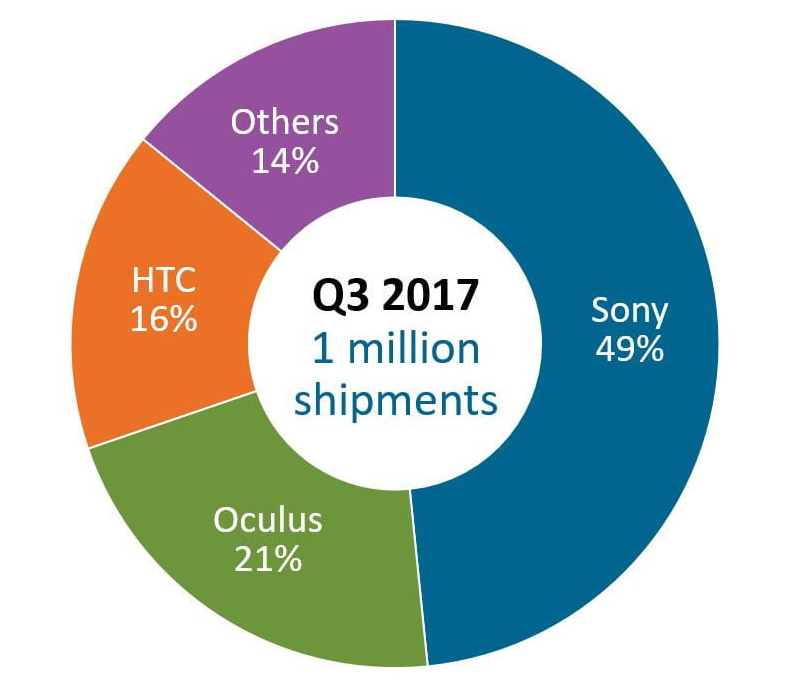
\includegraphics[scale=0.25]{pics/vr_headset_manufacturer_marketshare}
    \caption{Market-share VR Headset Hersteller~\cite{MARTINDALE_2017}}
    \label{fig:vr_headset_manufacturer_marketshare}
\end{figure}

\subsubsection{HTC Vive Pro}\label{sec:htc-vive}

Wie bereits in Abschnitt~\ref{sec:vr-headset-types} beschrieben, gibt es von diesen Headsets verschiedene Modelle.
Die HTC Vive Pro ist vom Typ ein tethered Headset mit dem Zusatz, dass auch sogenannte Light Houses gebraucht werden (siehe Abschnitt~\ref{sec:lighthouse_tracking}).
Andere Produkte, wie die im Folgendem beschriebene Oculus Quest benötigen solche nicht.

\paragraph{Vorteile}

\begin{itemize}
    \item die HTC kann mit SteamVR verwaltet werden, womit der manuelle Download von externer Software vermieden wird.
    \item lighthouse tracking
    \begin{itemize}
        \item genaueres tracking~\ref{fig:tracking_precision_statistic}
        \item nicht von dem natürlichen Licht abhängig~\cite{Dennis_Ziesecke_2019}
    \end{itemize}
\end{itemize}

\begin{figure}
    \centering
    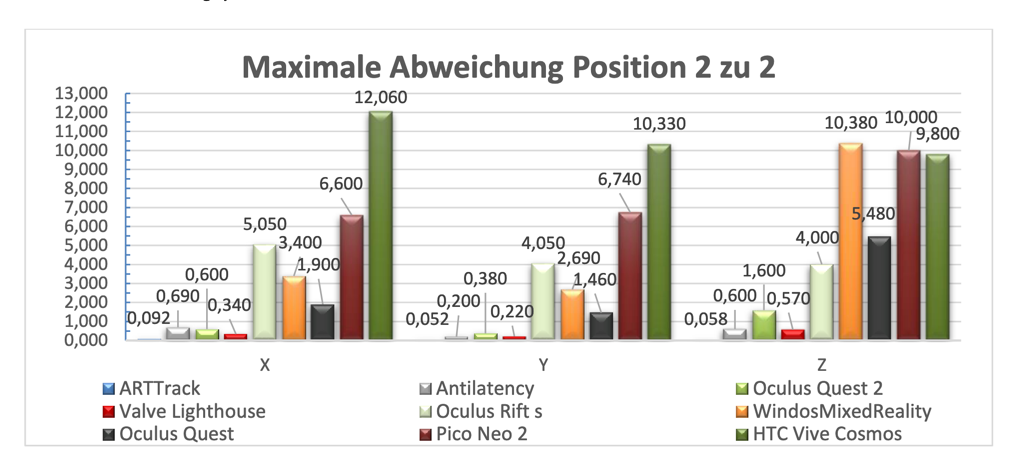
\includegraphics[scale=0.4]{pics/tracking_precision_statistic}
    \caption{Tracking Genauigkeit der VR Headsets~\cite{Macedo_2020}}
    \label{fig:tracking_precision_statistic}
\end{figure}

\paragraph{Nachteile}

\begin{itemize}
    \item längerer Aufbau wie die Folgend beschriebene Oculus Quest 2
    \item hoher Preis~\ref{fig:vr_headset_prices}
    \item es wird ein Computer benötigt
\end{itemize}

\begin{figure}
    \centering
    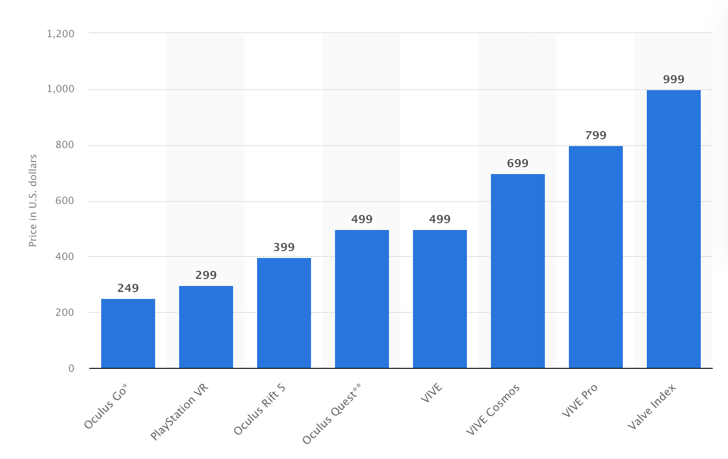
\includegraphics[scale=0.5]{pics/vr_headset_price_statistic}
    \caption{VR Headset Preise~\cite{ALSOP_2019}}
    \label{fig:vr_headset_prices}
\end{figure}

\subsubsection{Valve Index}

Die Valve Index ist eine VR-Brille welche von Valve entwickelt worden ist.
Diese befindet sich genauso wie die HTC Vive Pro~\ref{sec:htc-vive} im teureren Spektrum~\cite{ALSOP_2019} der VR-Brillen und ist dem Typ tethered Headset~\ref{sec:vr-headset-types} zuzuordnen.

\paragraph{Vorteile}

\begin{itemize}
    \item Hand Tracking.
    Die Controller tracken die Finger- und Handbewegungen.
    Diese Technologie kann von Spieleentwicklern verwendet werden~\cite{SadlyItsBradley_2019}
    \item lighthouse tracking (siehe HTC Vive)
\end{itemize}

\paragraph{Nachteile}

\begin{itemize}
    \item längerer Aufbau wie die Folgend beschriebene Oculus Quest 2
    \item hoher Preis~\ref{fig:vr_headset_prices}
    \item es wird ein Computer benötigt
\end{itemize}

\subsubsection{Oculus Quest 2}\label{sec:oculus-quest-2}

Die Oculus Quest 2 ist eine VR-Brille welche von Facebook/Meta im Jahre 2020 entwickelt worden is~\cite{ADI_ROBERTSON_2020}.
Diese Brille ist eine Mischung von einem tethered Headset und einem Standalone Headset~\ref{sec:vr-headset-types}.
Dies bedeutet, dass die Oculus Quest 2 ohne einen Computer benutzbar ist, aber auch mit einem USB-C Kabel zu einem Computer verbunden werden kann.
Ist das Headset mit dem Computer verbunden können PC exclusive Spiele mit der Oculus Quest 2 auch gespielt werden~\cite{ADI_ROBERTSON_2020}
Für den Aufbau werden nur das Headset und zwei Controller benötigt.

\paragraph{Vorteile}

\begin{itemize}
    \item Aufbauen erfordert keinen großen Aufwand.
    \item Die Brille befindet sich eher im unteren Preisspektrum der VR-Brillen~\ref{fig:vr_headset_prices}.
    \item es wird kein Computer benötigt
\end{itemize}

\paragraph{Nachteile}

\begin{itemize}
    \item Das Headset ist von natürlichem Licht abhängig~\cite{Dennis_Ziesecke_2019}
    \item Full Body Tracking kann etwas kompliziert und teuer werden~\cite{Martin_Rakver}
    \item weniger genaues Tracking~\cite{Macedo_2020}
\end{itemize}

\subsection{VR Controller}\label{sec:vr-controller}

\subsection{Tracker}\label{sec:tracker}

\subsubsection{Vive Tracker}\label{sec:vive-tracker}

\subsection{Lighthouse Tracking}\label{sec:lighthouse_tracking}

\subsubsection{Grundlagen}

Die HTC Vive Brillen und die Valve Index benützen beide das Lighthouse-Tracking~\cite{steam_lighhouse_versions}.
Diese Form des Trackings ist genauso wie das Tracking der Oculus Quest und Oculus Quest 2 (siehe~\ref{sec:oculus_quest_tracking, sec:oculus-quest-2}) ein Inside-Out Tracking.
Im Gegensatz zu der Oculus Quest benützt das Lighhouse Tracking kein natürliches Licht, sondern für das Auge unsichtbares Licht.
Diese Form des Tracking wird auch Marker-Based Inside-Out Tracking genannt\ref{sec:tracking}.
Im Falle des Lighhouse Tracking beleuchten die Base Stations die zu trackenden Geräte, womit sich die Geräte orientieren können.
Dies hat den Vorteil, dass die Benutzung der Vr Brille nicht von dem natürlichen abhängig ist.
Statt Kameras besitzt ein zu trackendes Gerät Fotosensoren~\cite{Buckley_2015}.

\subsubsection{Positionierung}

Damit dieser Vorgang fehlerfrei funktioniert werden typischerweise zwei Basestations verwendet
Diese werde wie in Abb~\ref{fig:basetstation_positioning} positioniert.
Mögliche Fehler können auftreten, wenn die Lighthouses keine klare Sicht auf die Geräte haben~\cite{steam_lighhouse_versions}..

\begin{figure}
    \centering
    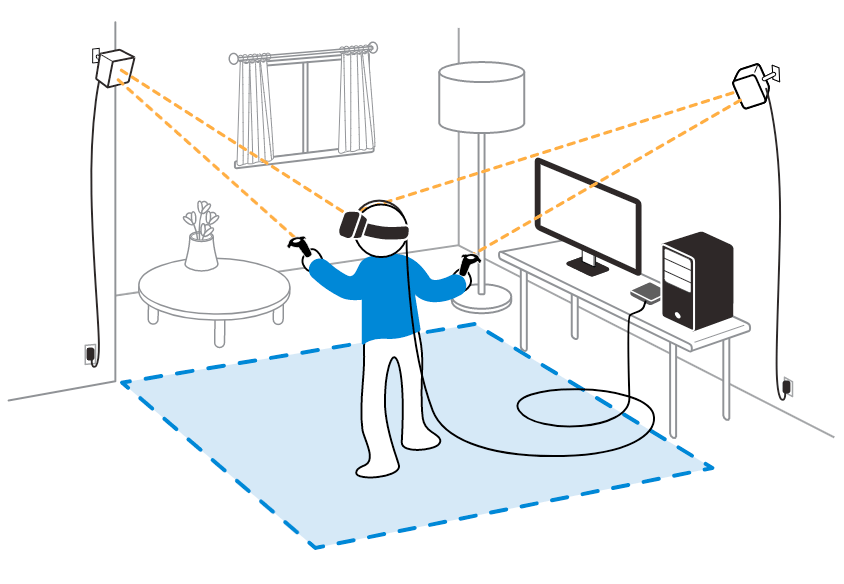
\includegraphics[scale=0.4]{pics/basestations_positioning}
    \caption{Positionierung der Lighhouses~\cite{Sercan_2018}}
    \label{fig:basetstation_positioning}
\end{figure}

\subsubsection{Funktionsweise}

Die Base Station besteht aus Syncblinker und Laseremitter.
Der Syncblinker ist ein Infrarot Strahl und die anderen 2 Laseremitter sind Lichtstrahlen welche sich 60-mal in der Sekunde auf einer Drehscheibe drehen.
Um die Position zu ermitteln, flasht der Sync Blinker und sobald dieser bei der Brille ankommt, fängt das Gerät zu zählen an bis die Lichtstrahlen der Laseremitter ankommen.
Durch die Drehscheibe, auf der sich die Laseremitter befinden, beleuchtet die Base Station so viele wie mögliche Sensoren.
Die Position mehrerer Punkte des Gerätes ist somit bekannt und es kann die Rotation der Brille ebenfalls berechntet werden~\cite{Buckley_2015, Skarredghost_2017}.

\subsubsection{Versionen}

Zum Zeitpunkt das Verfassen der Diplomarbeit gibt es 2 Versionen der Base Stations.
Version 1.0 und 2.0 sind nicht miteinander kompatibel.
Folgend sind die Versionen aufgelistet mit den jeweils kompatiblen Geräten in der Klammer.
Wobei Steam bei der Kompatibilität nur HTC Brillen und die Valve Index vermerkt haben, weshalb andere Brillen in der folgenden Liste ausgenommen worden sind~\cite{steam_lighhouse_versions}.

\begin{itemize}
    \item Lighthouse 1.0 (HTC Vive, Valve Index)
    \item Lighthouse 2.0 (HTC Vive Pro, Valve Index)
\end{itemize}

\emph{1.0 Lighthouses} besitzen eine nahezu quadratische form mit einer Länge von 15 cm, einer Breite von 16 cm und einer höhe von 10 cm

\emph{2.0 Lighthouses} haben einer eher rechteckige form mit einer Länge von 15 cm, einer Breite von 13,30 cm und einer Höhe von 12,90 cm.
Die Vorderseite ist der Länge nach abgerundet, mit welcher eine höhere Reichweite erreichbar is.
Mit der neuen Version ist es auch möglich mehrere Base Stations zu verwenden.
Durch die erhöhte Sichtweite und der Möglichkeit mehr wie zwei Lighthouses zu verwenden kann eine größere Spielfläche verwendet werden.
Der Sichtkontakt der Lighhouses ist nicht mehr nötig~\cite{Cale_2019}.


\subsection{Oculus Quest Tracking}
\label{sec:oculus_quest_tracking}

Eine weitere Art das Tracking wird benutzt von Oculus.
Wie bereits in~\ref{sec:lighthouse_tracking} erwähnt benutzt die Oculus Quest und Oculus Quest 2 ein Inside Out Tracking.
Die Oculus Quest benützt Kameras, um sich im VR Raum zu orientieren.

\subsubsection{DoF}

Es gibt zwei verschiedene Arten des Oculus Quest und Oculus Quest 2 Tracking zwischen denen das Headset wechseln kann.
Diese arten gelten nur für das VR Headset und nicht die Controller~\cite{oculus_support_headset_tracking}.

\begin{itemize}
    \item 3DoF
    \item 6Dof
\end{itemize}

\emph{3DoF} bedeutet, dass die Rotation des VR Headsets getracked werden.
Die Position wird nicht getracked.
Oculus empfehlt nur im Sitzen oder im Stehen zu spielen, wenn 3DoF aktiviert ist.

Bei \emph{6DoF} wird auch die Position getracked.
Viele Spiele setzen vorraus, dass die Position getracked wird.

\subsubsection{Headset Tracking}

Das Oculus Quest 2 Headset benützt ein etwas anderes Tracking.
Durch die Kameras, welche in dem Headset verbaut, sind analysiert es die Umgebung.
Mit Bildverarbeitung erstellt es es aus den aufgenommenen Bildern eine 3d Map.
Diese 3d Map wird benutzt um das Headset im dreidimensionalen Raum zu positionieren und rotieren~\cite{MECHATECH}.

\subsubsection{Controller Tracking}

Oculus nennt ihre virtual reality controller oculus touch.
Diese haben einen ring welcher einen Ring um die Hand Bilden, auf welchen sich eine Infrarot LED befindet.
Die Infrarot LED ist so positioniert, damit sie in die Richtung des Headsets schauen.
Parallel machen die Kameras, welche auf dem Headset sich befinden, Fotos.
Durch die Infrarot LED Strahlen kann das Headset mit den Fotos die Position der Controller ermitteln.
Das Infrarotlicht der Controller ist für das menschliche Aug nicht sichtbar~\cite{Gajsek_2022}.
Im Gegensatz zum Headsets benützen die Controller nach definition ein Outside in Tracking, da die Controller nicht von alleine wissen, wo sie sich im Raum befinden und das tracking mithilfe des Headset funktioniert.

\subsubsection{Guardian}

Oculus Guardian ist ein Sicherheitssystem, bei welchen man eine gewisse Spielfläche definieren kann.
Die Grenzen der Spielfläche werden dann angezeigt, wenn man sich diesen nähert~\cite{Oculus_Guardien}.

\emph{Guardian Space Sense} ist ein weiteres Sicherheitssystem.
Durch die 3d Map, welche schon in dem Abschnitt Headset Tracking beschrieben worden ist, kann auch eine Hilfestelle für den Nutzer geleistet werden.
Hier versuch die Oculus Quest Umrisse von Gegenständen, Menschen und anderen Lebewesen in der virtuellen realität sichtbar zu machen, wenn sich der Nutzer diesen nähert~\cite{Oculus_Guardien}.

\subsection{Wireless Adapter }

\section{Software}

\subsection{Game Engine}

Es gibt mehrere Games Engines mit welchen eine VR Applikation entwickelt werden kann.
In Abb.~\ref{fig:game_engine_marketshare} ist der Marktanteil verschiedener Engines abgebildet.
Diese Daten sind aber mit Vorsicht zu genießen, da das Skript welche diese Daten geliefert hat nach einigen Kriterien handelt,(siehe~\cite{REDDIT_2018}).
Dies bedeutet beispielsweise, dass nur Spiele mit einer Wikipedia Seite mit einberechnet werden.

\begin{figure}
    \centering
    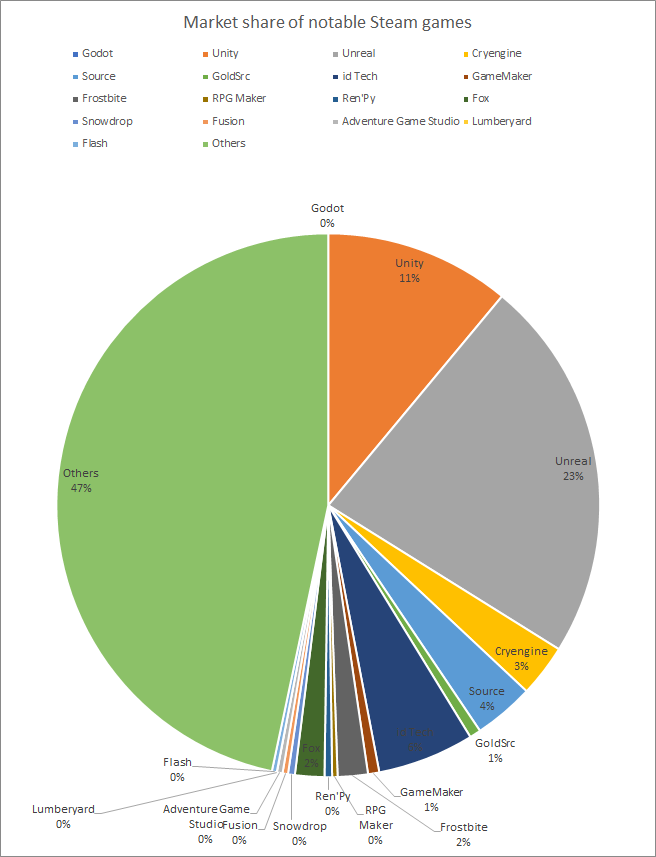
\includegraphics[scale=0.4]{pics/game_engine_marketshare}
    \caption{Game Engine Market-share~\cite{REDDIT_2018}}
    \label{fig:game_engine_marketshare}
\end{figure}

\begin{figure}
    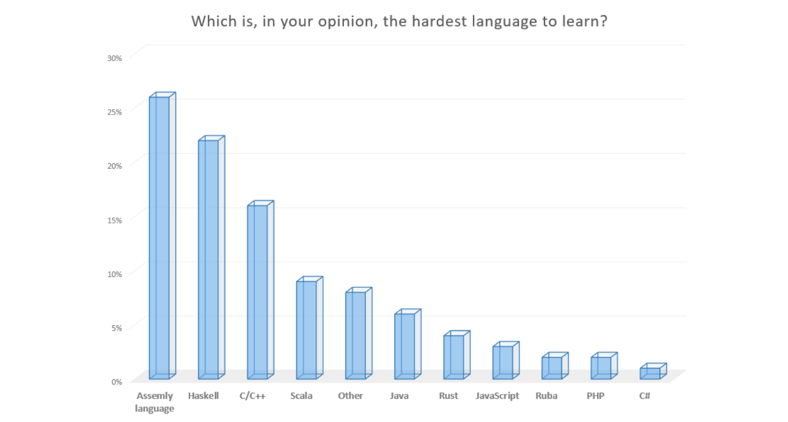
\includegraphics[scale=0.4]{pics/programming_languages_hardest}
    \caption{Schwerste Programmiersprachen~\cite{JAXCENTER_2018}}
    \label{fig:hardest_programming_languages}
\end{figure}

\subsubsection{Unity}

Unity ist eine Game Engine, welche von Unity Technologies initial exklusiv für Apple Mac OS X entwickelt wurde.
Die Engine wurde portiert und kann heute auch auf Windows und auf der Linux Plattform benützt werden.
Sie ist für alle im prinzip gratis bis zu einem bestimmten Umsatz.
Auch wenn sie eine Einsteiger Engine genannt wird, ist sie trotzdem im professionellen Bereich in benutzung und viele bekannte Spiele, wie Pokemon GO, Among us und Hearthstone wurden in der Unity Engine entwickelt~\cite{Haas2014AHO,UNITY_DOWNLOAD,UNITY_PRICING,WIKIPEDIA_UNITY_GAME_LIST_2014}.

\paragraph{Vorteile}

\begin{itemize}
    \item Gratis benutzung bis zu einem bestimmten Umsatz eines Produktes
    \item Programmierbar in C\#, einer einfach zu erlernenden Sprachen siehe Abb.~\ref{fig:hardest_programming_languages}
    \item Es kann für alle möglichen Plattformen ein Programm geschrieben werden~\cite{UNITY_PLATTFORMS}
    \begin{itemize}
        \item IOS
        \item Android
        \item Windows
        \item Linux
        \item WebGL
    \end{itemize}
\end{itemize}

\paragraph{Nachteile}

\begin{itemize}
    \item im Vergleich zu Unreal weniger Market-share~\ref{fig:game_engine_marketshare}
    \item geschlossener Source Code
    \item schnellerer Kostenanfall wie bei Unreal
\end{itemize}

\subsubsection{Unreal Engine}
\label{sec:unreal_engine}

Unreal Engine wird von Epic Games entwickelt~\cite{UNEAL_ENGINE_OWNER_2022}.
Diese Engine ist eine weit verbreitete Game Engine.
Dies kann man Abbildung~\ref{fig:game_engine_marketshare} entnehmen.
Viele Spiele wie Fortnite, Ark Survival Evolved, Borderlands 3 und Jedi Fallen Order sind mit dieser Engine entwickelt worden~\cite{WIKIPEDIA_UNREAL_GAME_LIST}.

\begin{figure}
    \centering
    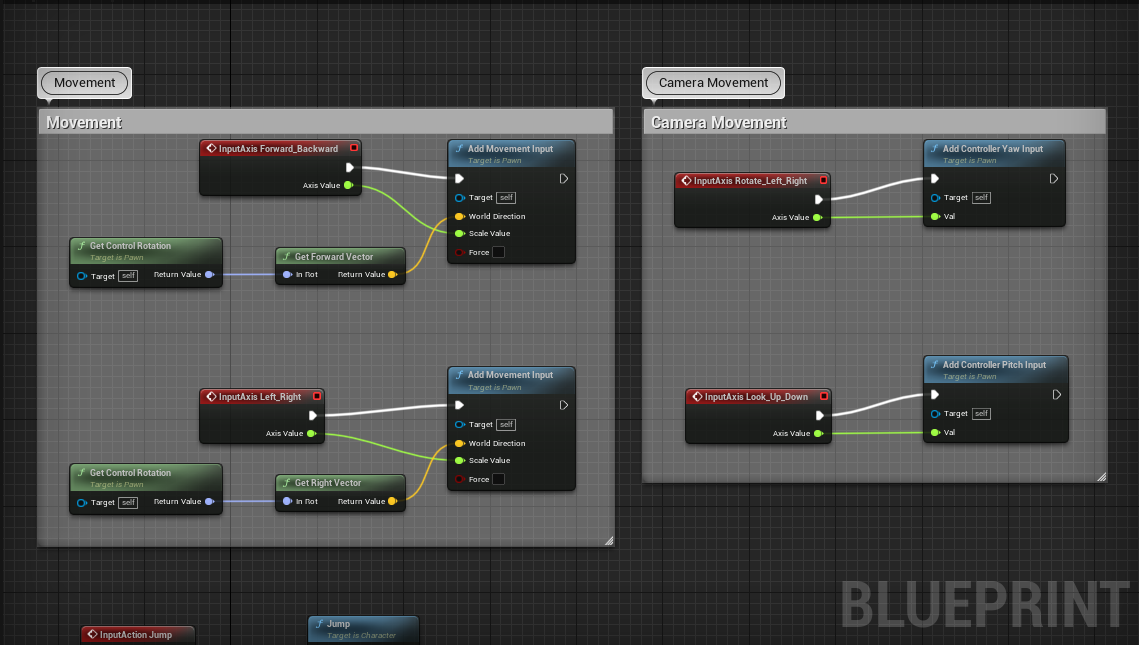
\includegraphics[scale=0.3]{pics/visual_scripting_unreal_engine}
    \caption{Visual Scripting in Unreal Engine 5}
    \label{fig:visual_scripting_unreal_engine}
\end{figure}

\paragraph{Vorteile}

\begin{itemize}
    \item höchster Market-share nach Abb.~\ref{fig:game_engine_marketshare}
    \item 'easy to learn' visual scripting~\ref{fig:visual_scripting_unreal_engine} %TODO: Statistic for visual scripting vs Code
    \item Lizenzkosten von 5\% folgen erst bei einem Einkommen durch ein Produkt von 1.000.000\$~\cite{UNREAL_ENGINE_PRICING_2022}
\end{itemize}

\paragraph{Nachteile}

\begin{itemize}
    \item 5\% Lizenzkosten, wenn das Einkommen eines Produktes über 1.000.000\$ ist~\cite{UNREAL_ENGINE_PRICING_2022}
    \item für erweiterte Funktionalität wird C++ benötigt, welches nach Umfrage in Abbildung~\ref{fig:hardest_programming_languages} die drittschwierigste Sprache zu erlernen ist
\end{itemize}

\subsubsection{Source Engine und Source 2 Engine}

Es gibt mittlerweile 2 Iterationen dieser Engine.
Zum einen die originale Source Engine und die Source Engine 2.
Die Markteinführung der ursprünglichen Source Engine war im Juni 2004~\cite{Bryan_Wirtz_SOURCE_ENGINE_2022}.
Daraufhin ist die Source 2 Engine im August 2014 erschienen~\cite{VALVE_DEVELOPER_COMMUNITY_SOURCE2}.
Beide Engines sind von Valve entwickelt worden~\cite{VALVE_DEVELOPER_COMMUNITY_SOURCE, VALVE_DEVELOPER_COMMUNITY_SOURCE2}.
Verantwortlich ist die Source 2 Engine für Spiele wie Dota 2 und Half Life Alyx~\cite{WIKIPEDIA_SOURCE2_ENGINE_GAME_LIST}.
Andere Spiele wie Half Life 2, Counterstrike Source, Portal, Portal 2 und Counterstrike Global Offensive sind mit der originalen Source Engine entwickelt worden~\cite{WIKIPEDIA_SOURCE_ENGINE_GAME_LIST}.
Auch als VR Entwicklungsumgebung eignet sich die Source 2 Engine, da sie für Half Life: Alyx, eines der erfolgreichsten VR Spiele benutzt worden ist~\cite{WIKIPEDIA_SOURCE2_ENGINE_GAME_LIST, Aden_Carter_2020}.
Die folgenden Vorteile und Nachteile beziehen sich auf die Source 2 Engine.

\paragraph{Vorteile}

\begin{itemize}
    \item Source Engine ist gratis zu nutzen und zu publizieren *(siehe Nachteile)
\end{itemize}


\paragraph{Nachteile}\label{pgr:cons}

\begin{itemize}
    \item kein hoher Market-share (siehe Abbildung~\ref{fig:game_engine_marketshare})
    \item spiele, welche mit der Engine entwickelt worden sind, dürfen nur auf Steam publiziert werden~\cite{Brenna_Hillier_2015}
\end{itemize}


\subsection{VR in Unity}
\setauthor{Florian Beckerle}
Unity bietet bereits eine eingebaute basis VR API, welche ein paar Features für die Verwendung von VR Geräten zur Verfügung stellt.
Diese muss jedoch erst Eingstellt werden, das geht in folgenden Schritten.

Um Vr für die Spiele zu aktivieren, müssen zuerst den Player Settings, welche im Menu bei Edit > Project Settings > Player zu finden sind, geöffnet werden.
Als nächstes muss die Option Virtual Reality Supported aktiviert werden, dass in der Box ein Häcken zu erkennen ist, siehe Abb. ~\ref{fig:unity_vr_api_settings}.
In der darunter stehenden Liste, namens Virtual Reality SDKs, können nun mit dem Plus-Knopf eine neue SDK hinzugefügt werden.
Ein Beispiel hierfür wäre die Oculus SDK.
Der Minus-Knopf bietet die Möglichkeit diese SDKs wieder zu entfernen, siehe Abb. ~\ref{fig:unity_vr_api_settings}.
~\cite{Unity_VR_Overview_2022}

Wenn VR aktiviert wurde, wird das Spiel automatisch auf die VR-Brille gerendert und dort angezeigt.
Weiters besitzt jede Kamera, welche im Spiel ist, eine Option, auf welches Auge das Ausgangsignal angezeigt werden soll, zum Beispiel linkes-, rechtes-, beide- oder keine Augen.
Unter den Augen versteht man die Bildschirme der VR-Brille welche sich vor den Augen des Benutzers befinden.
Ein weiteres automatisches Feature ist, dass die Bewegung der VR-Brille in der realtität auf die Position der Kamera im Spiel übertragen wird.

Unity empfielt für die verwendung der Api folgende Brillen, Gear VR, Oculus CV1 und die Vive.
~\cite{Unity_VR_Overview_2022}

\begin {figure}
    \centering
    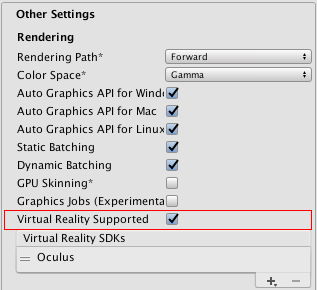
\includegraphics[scale=0.8]{pics/unity_basis_vr_api_settings}
    \caption{Unity VR API - Settings}
    \label{fig:unity_vr_api_settings}
\end {figure}

\subsection{VR Plugin}
\setauthor{Florian Beckerle}
Für BeamVR wurde das SteamVR Unity Plugin verwendet.
Es wurde von Valve entwickelt und bietet bereits eine Vielzahl an vorgefertigten Demos, welche mit der Installation des Plugins mitgeliefert werden, diese werden später genauer beschrieben..
~\cite{SteamVR_Overview_2022}

\subsubsection{Quickstart}
\setauthor{Florian Beckerle}
Für das Setup des SteamVR Unity Plugins sind 5 Schritte notwendig.
Damit alles Funktioniert muss SteamVR von Steam und das Plugin vom Unity Asset Store gedownloaded werden.
Nachdem die Installation beider Softwares abgeschlossen wurde, muss das Plugin, über den Package Manager, in das Unity Projekt importiert werden.
Im Menu Window wird nun eine neue Option namens SteamVR Input angezeigt, siehe Abb. ~\ref{fig:steamvr_input_menu_item}.
\begin {figure}
    \centering
    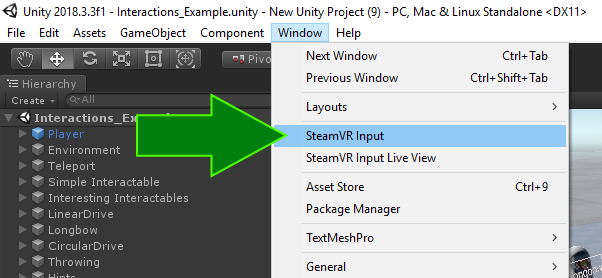
\includegraphics[scale=0.9]{pics/steamVR_Input_MenuItem}
    \caption{Steam VR - Input Menu Item}
    \label{fig:steamvr_input_menu_item}
\end {figure}
Wenn man auf diese klickt erscheint ein Popup welches fragt ob JSON Files kopiert werden sollen, dort drückt man auf Ja, siehe Abb. ~\ref{fig:steamvr_copy_json}.
\begin {figure}
    \centering
    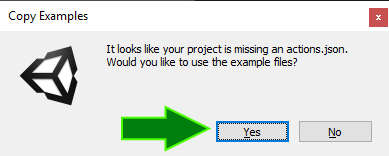
\includegraphics[scale=1]{pics/steamVR_Input_CopyJSON}
    \caption{Steam VR - Copy JSON}
    \label{fig:steamvr_copy_json}
\end {figure}
Nachdem der Vorgang abschlossen ist, öffnet sich das SteamVR Input Fenster, dort muss nun Save and Generate gedrückt werden, siehe Abb. ~\ref{fig:steamvr_save_and_generate}.
\begin {figure}
    \centering
    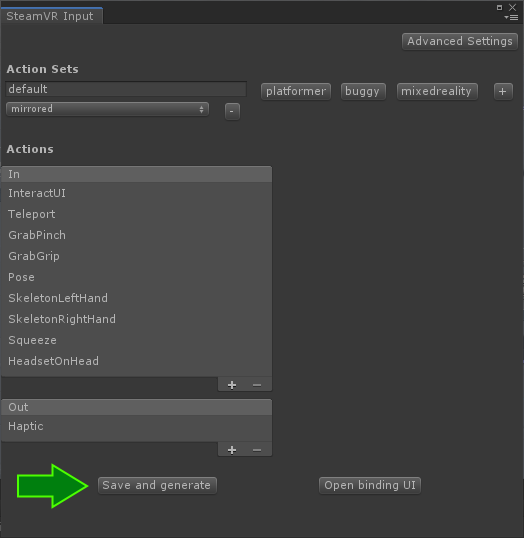
\includegraphics[scale=0.6]{pics/steamVR-Input-SaveAndGenerate}
    \caption{Steam VR - Save and Generate}
    \label{fig:steamvr_save_and_generate}
\end {figure}
Nun ist die Installation abgeschlossen und das SteamVR Unity Plugin ist einsatzbereit.
~\cite{SteamVR_Quickstart_2022}

\subsubsection{Render Models}
\setauthor{Florian Beckerle}
Das SteamVR Unity Plugin bietet eine virtuelle Darstellung der Kontroller, welche der Benutzer in den Händen hält.
Die gezeigten Modelle benötigen hierfür mehrere Attribute, siehe Abb. ~\ref{fig:steamvr_render_models Script}.
\begin {figure}
    \centering
    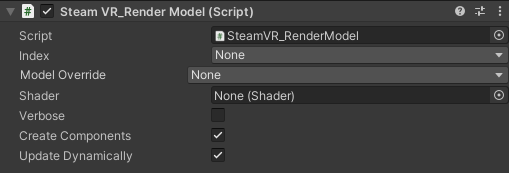
\includegraphics[scale=1]{pics/steamVR_render_models_script}
    \caption{Steam VR - Render Models Script}
    \label{fig:steamvr_render_models Script}
\end {figure}
Der Index ist der Index des getrackten Gerätes, und wird vom System wie eine ID zur Erkennung verwendet.
Mittels dem Model Override kann man für Testzwecke ein bestimmtes Modell festlegen welches angezeigt werden soll.
Die Shader können die Darstellung des Objektes verändern.
Verbose gibt die Vorgänge im Script in der Konsole aus, diese Option wird jedoch nur für das Testen benötigt.
Create Components erstellt individuelle Objekte für jeden Komponenten welcher verfügbar ist.
Update Dynamically bewegt die einzelnen Komponenten gleich wie die physischen Gegenstücke.
~\cite{SteamVR_Render_Models_2022}

\subsubsection{Input}
\setauthor{Florian Beckerle}
Die die Hardware für VR Geräte schnell weiterentwickelt wird, hat Valve auf ein KeyBinding System zurückgegriffen.
Die Entwickler und die Benutzer selbst können für neue oder breits vorhandene Hardware einstellen, welche Funktion die einzelnen Knöpfe und Trigger haben.
Diese Aktionen wurden in 6 verschiedene Input Typen und einen Output Typen  aufgeteilt.

Die Aktion Boolean besitzt zwei Zustände, true und false.
Sie wird oft benutzt um Objekte zu greifen, da man zum Beispiel einen Würfel entweder aufheben können soll oder nicht.

Single Aktionen können analoge Werte zwischen 0 und 1 annehmen und wird für Situationen benutzt wo der Boolean nicht ausreicht.
Ein Anwendungsfall ist ein Auto, welches bei 0 stehen bleibt und bei 1 Vollgas fährt.
Als Eingabe kann zum Beispiel der Trigger des Kontrollers benutzt werden.

Vector2 besitzt zwei Werte, X und Y.
Die Bewegungen des Kontrollers werden hierbei nur auf zwei Achsen gemessen.

Vector3 besitzt im Gegensatz zu Vector2 drei verschiedenen Werte X, Y und Z.
Diese Aktion wird selten benutzt, findet aber zum Beispiel im SteamVR Home einen Anwendungsfall beim Scrollen.

Pose gibt die Position und Rotation in einem dreidimensionalen Raum wieder.
Es wird dazu benutzt um die Bewegungen der Controller zu messen und digital nachzubilden.

Skeleton benutzt das SteamVR Skeleton Input um die ungefähre Position und Rotation der Finger zu erkennen, während der Kontroller in den Händen gehalten wird.

Vibration werden für haptisches Feedback bei VR Geräten verwendet.
Hierbei vibrieren der Kontroller, eine spezielle Haptik Weste oder ein preparierter Sessel.
~\cite{SteamVR_Input_2022}

\subsubsection{Skeleton Input}
\setauthor{Florian Beckerle}
Das Plugin bietet die Möglichkeit Hände mit Fingern und deren aktuellen Position darzustellen.
Die Bewegungen werden hierbei zwischen zwei verschiedenen Begränzungen der Fingerpositionen unterschieden.
WithContoller berechnet eine ungefähre Position der Finger während diese einen Kontroller in den Händen halten.
Dies dient besonders dazu, die Interaktion zwischen der realen Hand und dem realen Kontroller digital darzustellen.
WithoutController bietet die Bewegungen von Fingern, wenn sie keinen Kontroller in der Hand halten.
In der realtität kann währenddessen jedoch trotzdem ein Kontroller gehalten werden, es wird nur digital nicht angezeit, siehe Abb. ~\ref{fig:steamvr_skeletal_input_models}.
\begin {figure}
    \centering
    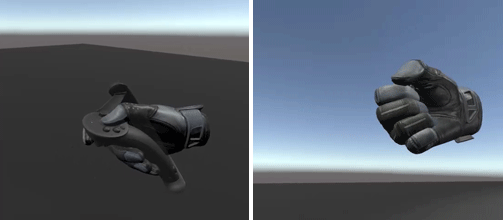
\includegraphics[scale=1]{pics/steamVR_skeletal_input_models}
    \caption{Steam VR - Skeletal Input Models}
    \label{fig:steamvr_skeletal_input_models}
\end {figure}
Die Positionen der Finger werden Relativ zu dem in der Hirarchie übergestuften Objekt und dem Model gemessen.
Jeder Finger besteht hierbei standardmäßig aus 4 Gelenken.
Ein Wert im Bereich von 0 bis 1 gibt an wie stark die Finger eingerollt sein sollen.
Die Finger einer Hand sind bei SteamVR etwas auseinander gestpeizt, hier wird ebenfalls ein Wert von 0 bis 1 dazu verwendet um die distanz zwischen den Fingern zu verändern.

Um die Position der Finger zu messen gibt es grunsätzlich drei verschiedene Methoden.
Bei Estimated kann die Position des Körperteiles nicht direkt bestimmt werden.
Jede Bewegung wird nur über die Bediehung der Trigger, Knöpfe und Trackpads des Kontrollers gestimmt.
Partial kann die bewegungen der Finger direkt bestimmen, jedoch nur eingeschränkter als wie die tatsächlichen Finger.
Die Positionen werden durch andere Werte, wie zum Beispiel von speziellen Handschuhen, gemessen.
Full kann die komplette Körperbewegung des Benutzers messen, wie zum Beispiel durch Motion Caputre Anzügen oder handschuhen.

Das Script, welches für die Bewegung des Modelles zuständig ist, besitzt eine Vielzahl an verschiedenen Optionen, siehe Abb. ~\ref{fig:steamvr_skeletal_input_Script}.
Update Pose setzt die Position und Orientierung des Objektes neu, sobald der Controller bewegt wurde.
Mirroring gibt an, ob die Knochen Daten entlang der X-Achse gespiegelt werden sollen.
Die Blend Optionen bieten Einstellungsmöglichkeiten den Übergang zwischen Verschiednen Bewegungsmöglichkeiten und Animationen zu verändern.
Weiters kann man einen bestimmten Knochen mittels GetBonePosition bekommen und die Positionen und Rotationen werden bittels GetBonePositions und GetBoneRotations bereitgestellt.
\begin {figure}
    \centering
    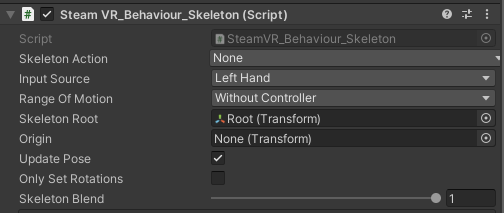
\includegraphics[scale=1]{pics/steamVR_skeletal_input_script}
    \caption{Steam VR - Skeletal Input Script}
    \label{fig:steamvr_skeletal_input_Script}
\end {figure}
~\cite{SteamVR_Skeleton_Input_2022}

\subsubsection{Interaction System}
\setauthor{Florian Beckerle}
Das Interaction System funktioniert mittels dem Senden von Nachrichten an Objekte, mit welchen die Hände des Spielers oder andere Objekte interagieren.
Diese Objekte können sich an die Hand anheften und somit gehalten werden.
Das System bietet die Möglichkeit Maus Events nachzuahmen, somit funktioniert die interaktion mit der Benutzeroberfläche auch in VR.

Die Player Klasse weiß wo die VR-Brille und die Kontroller positioniert sind.
Mittels den Methoden hmdTransform und feetPositionGuess können die Positionen der Brille und eine schätzung der Fußstellung zurückgeliefert werden.

Die Hand Klasse wird für die meißten Funktionen des Interaction Systems benötigt.
Sie sendet interagierbaren Objekten Nachrichten über den aktuellen Status der Hand.
Sie kann nur mit einem Objekt gleichzeitig direkt Interargieren, darunter versteht man das aufheben und werfen dieser.
Objekte können an die Hand angebracht und wieder losgelöst werden.
Das Verhalten der Hände kann durch sogenannte AttachmentFlags veränder werden, welche bei einer Interaktion aktiviert werden.

Interactable Objekte können von Spielern aufgehoben werden, solange ein bestimmter Knopf gedrückt wird.
Befindet sich die Hand, während dieser Knopf losgelassen wird, in Bewegung wird die Geschwindigkeit und die Richtung auf das Objekt übertragen und es wird geworfen.
%%Optional noch andere Scripts erklären falls notwendig, erscheinen jedoch nicht sonderlich wichtig (wichtigere noch mit !)
%    Throwable
%    LinearDrive
%    CircularDrive
%    LinearMapping
%    VelocityEstimator !!
%    IgnoreHovering
%    UIElement
%    ItemPackage
%    ItemPackageSpawner
%    ItemPackageReference
%    PlaySound
%    SoundPlayOneShot
%    Util
%    InteractableHoverEvents
%    InteractableButtonEvents
%    ComplexThrowable
%    DistanceHaptics
%    Player (Prefab) !!
%    BlankController (Prefab)
%    Teleport !!
%    Render Model
%    Hints
%    Samples
~\cite{SteamVR_Interaction_System_2022}

\subsubsection{Skeleton Poser}
\setauthor{Florian Beckerle}
Der Skeleton Poser funktioniert mithilfe von verschienen Posen, welche erstellt und eingefügt werden können.
Mittels dem Blending Editor des Posers kann zwischen verschiedenen Posen ein Übergang erstellt werden.

Hierbei existieren 4 Modi für die Fingerbewegungen.
Der Static Modus erlaubt keine Fingerbewegungen und beachtet nur die Posen.
Bei Free können die Finger frei bewegt werden und die Pose wird ignoriert.
Mittels Extend können die Finger komplett ausgestreckt werden, aber nur nicht weiter eingerollt werden, als es bei der Pose eingestellt wurde.
Bei Contract können die Finger ganz eingerollt werden, jedoch nicht weiter Ausgestreckt werden als bei der Pose.
~\cite{SteamVR_Skeleton_Poser_2022}

OpenVR Plugin
\subsubsection{OpenVR}
OpenVR ist eine API, welche den direkten Zugriff auf VR-Hardware von verschiedenen Anbietern, wie Oculus, Mixed Reality und Vive, ermöglicht.
Hierbei benötigt die Anwendung keine speziellen Kenntnisse über die Hardware.
OpenVr besteht aus der Applikation und dem Treiber, welche über SteamVR miteinander kommunizieren.
Die API besteht aus mehreren C++ Interface Klassen.
Wenn die Applikation ausgeführt wird, liefert OpenVR, je nach vorhandenem SDK, das benötigte Interface zurück.
~\cite{OpenVR_Github_Documentation_2020}

\subsubsection{OpenVR Treiber}

~\cite{OpenVR_SteamWorks_Documentation_2020}


\subsection{SteamVR}

\subsection{Vive Wireless}

\subsection{Final IK Plugin}
\subsubsection{Aim IK}
\subsubsection{Arm IK}
\subsubsection{Baker}
\subsubsection{Bipaed IK}
\subsubsection{CCD IK}
\subsubsection{FABRIK}
\subsubsection{FABRIK IK}
\subsubsection{Full Body Biped IK}
\subsubsection{Grounder}
\subsubsection{Interaction System}
\subsubsection{Leg IK}
\subsubsection{Limb IK}
\subsubsection{Look At IK}
\subsubsection{Rotation Limits}
\subsubsection{Trigonometric IK}
\subsubsection{VRIK}
\subsubsection{Extending Final IK}


\subsection{IDE}

\subsection{Modellierung}
